\documentclass[11pt]{article}
% \def\hidesolutions{}
%%%%%%%%%%% SET MARGINS
\setlength{\textheight}{20cm}
\setlength{\topmargin}{-0.5cm}
\setlength{\oddsidemargin}{+0cm}
\setlength{\textwidth}{16.3cm}
%\setlength{\parskip}{6pt}
\setlength{\parindent}{0pt}

%%%%%%%%%%% PACKAGES
\usepackage{amsmath}
\usepackage{amssymb}
\usepackage{amsfonts}
%\usepackage{a4wide}
\usepackage{graphicx}
\usepackage{color}
\usepackage[normalem]{ulem}
\usepackage{enumitem}
\usepackage{capt-of}
\usepackage{float}
\usepackage{amsmath}
\usepackage{listings}
\definecolor{mygreen}{RGB}{28,172,0} % color values Red, Green, Blue
\definecolor{mylilas}{RGB}{170,55,241}
\usepackage{empheq}
\usepackage[ruled]{algorithm2e}
\usepackage{mathrsfs}
\usepackage{datetime}
\usepackage{subcaption}

% TODO: combine the two package lists and reduce redundancies 
\usepackage{mathtools}
\usepackage{nicefrac}
\usepackage{hyperref}
\usepackage{url}
\usepackage{amsmath,amssymb,amsfonts}
\usepackage{a4wide}
\usepackage{graphicx}
\usepackage{color}
\usepackage[normalem]{ulem}
\usepackage{capt-of}
\usepackage{float}
\usepackage[ruled]{algorithm2e}
\usepackage{amsmath,amssymb,amsfonts}
\usepackage{a4wide}
\usepackage{graphicx}
\usepackage{color}
\usepackage[normalem]{ulem}
\usepackage{capt-of}
\usepackage{float}
\usepackage[ruled]{algorithm2e}
\usepackage{mathrsfs}







\newcommand{\Lc}[2]{{\color{blue} \sout{#1} } \textcolor{red}{#2}}
\newcommand{\La}[1]{\textcolor{red}{#1}}
\newcommand{\lh}{\mathscr{L}_h}
\newcommand{\cl}{\mathscr{L}}
\newcommand{\cf}{\mathscr{F}}
\newcommand{\dx}{dx}
\newcommand{\ltn}{\mathscr{l}^2}
\newcommand{\bbR}{\mathbb{R}}
\newcommand{\Rset}{\mathbb{R}}
\newcommand{\Nset}{\mathbb{N}}
\newcommand{\scL}{\mathcal{L}}
\newcommand{\xx}{\mathbf{x}}
\newcommand{\norm}[1]{\|{#1}\|}
\newcommand{\yy}{\mathbf{y}}
\newcommand{\at}[1]{\big|_{#1}}
\renewcommand{\div}{\mathrm{div}}
\newcommand{\divergence}{\mathrm{div}}
\newcommand{\cp}[1]{\textcolor{blue}{#1}}

\newcommand{\FF}{\texttt{FreeFem++ }}
\newcommand{\FFns}{\texttt{FreeFem++}}
\newcommand{\FFfull}{\texttt{FreeFem++-x11}}
\newcommand{\cmd}[1]{ \medskip \noindent \texttt{#1} \medskip}
\newcommand{\incmd}[1]{\texttt{#1}}
\newcommand{\shrinkitems}{\addtolength{\itemsep}{-0.5\baselineskip}}
\newcommand{\mtt}[1]{\mathtt{#1}}
\newcommand{\ML}{\texttt{Matlab }}

\newcommand{\bb}{\mathbf{b}}
\newcommand{\nn}{\mathbf{n}}
\newcommand{\vecA}{\vec{A}}
\newcommand{\vecB}{\vec{B}}


\newcommand{\mesh}{\mathcal{T}_h}
\newcommand{\refel}{\widehat{K}}
\newcommand{\ver}{\mathbf{a}}
\newcommand{\refver}{\widehat{\mathbf{a}}}
\newcommand{\grad}{\nabla}
\newcommand{\refgrad}{\widehat{\nabla}}
\newcommand{\refu}{\widehat{u}}
\newcommand{\refbasis}{\widehat{\varphi}}
\newcommand{\refxx}{\widehat{\xx}}
\newcommand{\refx}{\widehat{x}}
\newcommand{\refy}{\widehat{y}}
\newcommand{\refrho}{\widehat{\rho}}
\newcommand{\refh}{\widehat{h}}






% For typesetting Python code
\newcommand{\matlab}{{\sc Matlab}\xspace}
\usepackage{listings}
\lstloadlanguages{Python}
\lstloadlanguages{csh}%
\definecolor{MyDarkGreen}{rgb}{0.0,0.4,0.0}
\definecolor{purple}{rgb}{0.58,0,0.82}
\lstset{language=Python,                    % Use Python
	%frame=single,                          % Single frame around code
	basicstyle=\ttfamily\footnotesize\color{black},
	keywordstyle=[1]\color{blue}\bf,        % Python functions bold and blue
	keywordstyle=[2]\color{purple},         % Python function arguments purple
	keywordstyle=[3]\color{red}\underbar,   % User functions underlined and blue
	commentstyle=\usefont{T1}{pcr}{m}{sl}\color{MyDarkGreen}\small,
	stringstyle=\color{purple},
	showstringspaces=false,                 % Don't put marks in string spaces
	tabsize=3,                              % 5 spaces per tab
	morekeywords={xlim,ylim,var,alpha,factorial,poissrnd,normpdf,normcdf},
	morecomment=[l][\color{blue}]{...},
	breaklines=true,
	breakatwhitespace=true,
	emptylines=1,
	mathescape=true,
	xleftmargin=0ex,
	emphstyle=\bfseries\color{red}
}





%%%%%%%%%%% MACROS NAMES
\newcommand{\lecturername}{Martin Licht}
% \newcommand{\assistantnamea}{Jochen Hinz}
% \newcommand{\assistantnameb}{Ivan Bioli}
\newcommand{\semestername}{Winter Semester 2023}
\newcommand{\lecturename}{Analysis III - 202(c)}
\DeclarePairedDelimiter\floor{\lfloor}{\rfloor}

%%%%%%%%%%% HEADER
\newdateformat{yeardate}{\THEYEAR}
\newcommand{\exsheet}[3] % input is the number of the session and the day TODO What's that
{\clearpage

	\begin{center}
		{\Large \textbf{\lecturename}}\\[2ex]
		\semestername
	\end{center}

	% \vspace{2ex}
	% \lecturername

	\vspace{2ex}
	{\Large Session #1: #3\,#2, \yeardate\today}
	%\hfill
	%{\Large EPF Lausanne}

	\hrulefill
}





\usepackage{comment}

\newtheorem{exercise}{Exercise}
\newtheorem{solutionenv}{Solution}

\newboolean{hide_solution}
\ifx\hidesolutions\undefined
\newenvironment{solution}{\begin{solutionenv}}{\end{solutionenv}}
\setboolean{hide_solution}{false}
\else
\excludecomment{solution}
\setboolean{hide_solution}{true}
\fi

\newcommand{\ifnotsolution}[1]{\ifthenelse{\boolean{hide_solution}}{#1}{}}
\newcommand{\ifsolution}[1]{\ifthenelse{\boolean{hide_solution}}{}{#1}}








\allowdisplaybreaks

\begin{document}
\exsheet{9}{14}{November} % parameters are the number of the session and the day


\begin{exercise}
 
Show that 
\begin{align}
    \int_{-\infty}^{\infty} e^{-x^2} \, dx = \sqrt{\pi}. 
\end{align}
\textit{Hint: square the integral and convert it to polar/radial coordinates.}
\end{exercise}
\begin{solution}
    Following the hint, we find
    \begin{align}
        \left(\int_{-\infty}^\infty e^{-x^2} dx\right)^2 &= \int_{-\infty}^\infty e^{-x^2} dx \int_{-\infty}^\infty e^{-y^2} dy = \int_{-\infty}^\infty \int_{-\infty}^\infty e^{-(x^2 + y^2)} dx dy\\
        &= \int_0^{2\pi} \int_0^\infty e^{-r^2} r dr d\theta = 2\pi \int_0^\infty e^{-r^2} r dr \\
        &= \pi \int_0^\infty e^{-u} du = \pi [-e^u]_0^\infty = \pi,
    \end{align}
    where we have used the substitution $u = r^2$ and Fubini's Theorem. Taking the square root of both sides gives the desired result.
\end{solution}


\begin{exercise}
    \begin{itemize}    
        \item 
        Show that 
        \begin{align}\label{eq:ex2 dist1}
            T(\phi) = \int_{-1}^{1} \phi(x) \ dx
        \end{align}
        is a distribution. 
        \item 
        Show that 
        \begin{align}\label{eq:ex2 dist2}
            T(\phi) = \int_{-\infty}^{\infty} \phi(x) \ dx
        \end{align}
        is a distribution. 
        \item 
        Show that 
        \begin{align}\label{eq:ex2 dist3}
            S(\phi) = \int_{0}^{1} |\phi(x)| \ dx 
        \end{align}
        is not a distribution.
    \end{itemize}
\end{exercise}
\begin{solution}
    The definition in \eqref{eq:ex2 dist1} is clearly linear in $\phi$ as the integral is linear
     and finite for any $\phi \in \mathcal{D}$ since continuous functions on compact sets are bounded. In particular, we have
     \begin{align}
            |T(\phi)| = \left| \int_{-1}^{1} \phi(x) \ dx \right| \leq \int_{-1}^{1} |\phi(x)| \ dx \leq \sup_{x \in [-1,1]} |\phi(x)| \int_{-1}^{1} dx = 2 \sup_{x \in [-1,1]} |\phi(x)|,
     \end{align}
     which proves the continuity.\\

    The definition in \eqref{eq:ex2 dist2} is also linear in $\phi$ for the same reason as before. To show that the integral is finite for any $\phi \in \mathcal{D}$, we use the fact that $\phi$ is compactly supported and hence bounded.
     In particular, there exists for any $\phi \in \mathcal{D}$ a compact interval $[a, b] \subset \mathbb{R}$ such that $\mathrm{supp}(\phi) \subset [a, b]$. Then we have
    \begin{align}
        |T(\phi)| = \left| \int_{-\infty}^{\infty} \phi(x) \ dx \right| \leq \int_{a}^{b} |\phi(x)| \ dx \leq \sup_{x \in [a,b]} |\phi(x)| \int_{a}^{b} dx = (b-a) \sup_{x \in [a,b]} |\phi(x)| < \infty,
    \end{align}
    which shows that the integral is finite for any $\phi \in \mathcal D$. Conversely, for any compact interval $[a, b] \in \mathbb{R}$ and $\phi \in \mathcal{D}$, such that $\mathrm{supp}(\phi) \subset [a, b]$, we have
    \begin{align}
        |T(\phi)| = \left| \int_{-\infty}^{\infty} \phi(x) \ dx \right| \leq \int_{a}^{b} |\phi(x)| \ dx \leq \sup_{x \in [a,b]} |\phi(x)| \int_{a}^{b} dx = (b-a) \sup_{x \in [a,b]} |\phi(x)|,
    \end{align}
    which shows the continuity.
    \\

    The definition in \eqref{eq:ex2 dist3} is not a distribution since it is not linear in $\phi$. 
    To see this, consider $\phi \in \mathcal{D}$ such that $\phi(x) \geq 0$ for all $x \in \mathbb{R}$. Set $\psi = -\phi \in \mathcal D$. Then we have
    \begin{align}
        S(\phi + \psi) = \int_0^1 |\phi(x) + \psi(x)| \ dx = \int_0^1 0 \ dx = 0,
    \end{align}
    but
    \begin{align}
        S(\phi) + S(\psi) = \int_0^1 |\phi(x)| \ dx + \int_0^1 |\psi(x)| \ dx = 2 \int_0^1 |\phi(x)| \ dx > 0.
    \end{align}
\end{solution}


\begin{exercise}
    Suppose that $f : \mathbb R \rightarrow \mathbb R$ is an integrable function. 
    Whenever $a > 0$, show that 
    \begin{align}
        \langle f, \phi \rangle := \frac{1}{a} \langle f, \phi(a \cdot) \rangle 
    \end{align}
\end{exercise}
\begin{solution}
    With the substitution $u = ax$, hence $du = a dx$, we find 
    \begin{align}
        \langle f(u) \phi(u/a) \frac 1 a \ d u
        = 
        \langle f(ax) \phi(x) \ d x 
        .
    \end{align}
    The desired result follows. 
\end{solution}



\begin{exercise}
    Find the distributional derivative of the function 
    \begin{align}
        f(x) = |x|.
    \end{align}
\end{exercise}
\begin{solution}
    Denote by $H(x)$ the Heaviside step function, where
    \begin{align}
        H(x) = \begin{cases}
                0 & \text{ if } x < 0 \\
                1 & \text{ if } x \geq 0.
               \end{cases}
    \end{align}
    We claim that $f' = 2 H - 1$ in the sense of distributions. Indeed, for a test function $\phi \in \mathcal{D}$,
     we have by definition of the distributional derivative that
    \begin{align}
        \langle f', \phi \rangle &= - \langle f, \phi' \rangle = - \int_{-\infty}^{\infty} |x| \phi'(x) \ dx = - \int_0^\infty x \phi'(x) \ dx + \int_{-\infty}^0 x\phi'(x) \ dx \\
        &= -[x \phi(x)]_0^\infty + \int_0^\infty \phi(x) \ dx + [x \phi(x)]_{-\infty}^0 - \int_{-\infty}^0 \phi(x) \ dx \\
        &= \int_0^\infty \phi(x) \ dx - \int_{-\infty}^0 \phi(x) \ dx = 2 \int_0^\infty \phi(x) \ dx - \int_{-\infty}^{\infty} \phi(x) \ dx = \langle 2H - 1, \phi \rangle,
    \end{align}
    where we have used that $\phi$ is compactly supported and hence the boundary terms vanish. This shows that $f' = 2H - 1$ in the sense of distributions.
\end{solution}


\begin{exercise}
    Consider the function with period $2$ that satisfies 
    \begin{align}
        f(x) = \begin{cases}
                -x & \text{ if } -1 < x \leq 0 \\
                 x & \text{ if }  0 < x \leq 1 \\
               \end{cases}
    \end{align}
    \begin{itemize}
     \item Draw a plot of this function from $-4$ to $4$.
     \item Is this function differentiable? What is the first distributional derivative of this function?
     \item What is the second distributional derivative of this function?
    \end{itemize}
\end{exercise}
\begin{solution}
    \begin{figure}
    \centering
    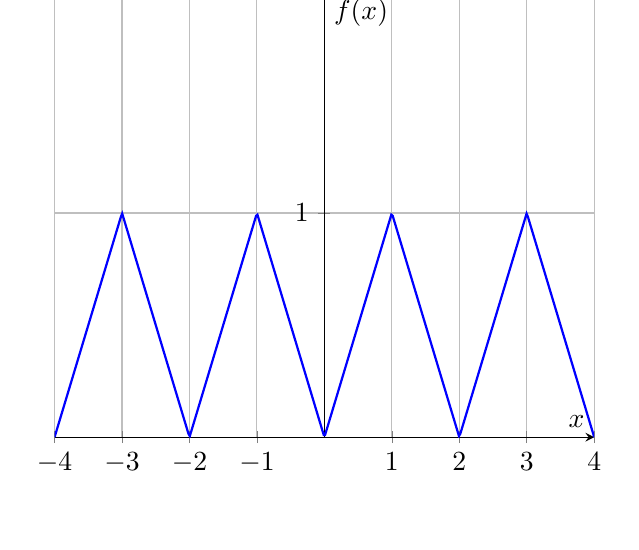
\begin{tikzpicture}
        \begin{axis}[
            axis lines=middle,
            xlabel={$x$},
            ylabel={$f(x)$},
            xmin=-4, xmax=4,
            ymin=0, ymax=2,
            samples=400,
            domain=-4:4,
            xtick={-4,-3,...,4},
            ytick={-1, 0, 1},
            grid=major
        ]
        % Plot the piecewise periodic function
        \addplot[thick, blue, domain=-4:4] 
            {(mod(abs(x), 2)) * (mod(abs(x), 2) <= 1) + (2 - mod(abs(x), 2)) * (mod(abs(x), 2) > 1)};
        \end{axis}
    \end{tikzpicture}
    \caption{Plot of the periodic function $f$.}
    \label{fig:ex5}
    \end{figure}
    The solution is plotted in Figure \ref{fig:ex5}. The function is not differentiable at $x \in \mathbb{Z}$ since the left and right derivatives do not agree.
     To compute the distributional derivative, we first observe that 
    \begin{align}
        f(2n) = 0, & & f(2n + 1) = 1, & & f(2n - 1) = -1 & & \forall n \in \mathbb{Z}.
    \end{align}
    Furthermore, we have that
    \begin{align}
        f'(x) = \begin{cases}
                -1 & \text{ if } x \in [2n - 1, 2n) \\
                 1 & \text{ if }  \in [2n, 2n + 1) \\
                \end{cases}, & & \forall n \in \mathbb{Z}.
    \end{align}
    Finally, for any $\phi \in \mathcal{D}$, there exists $N \in \mathbb{N}$ such that $\mathrm{supp}(\phi) \subset [-2N, 2N]$.\\
    We claim that $f' = 2 \sum_{n \in \mathbb{Z}} 1_{[2n, 2n + 1)} - 1$ in the sense of distributions, where $1_{[a,b)}$ denotes the indicator function of the interval $[a,b)$.
    Indeed, for a test function $\phi \in \mathcal{D}$, we have by definition of the distributional derivative that
    \begin{align*}
        \langle f', \phi \rangle &= - \langle f, \phi' \rangle = - \int_{-\infty}^{\infty} f(x) \phi'(x) \ dx = - \sum_{n \in \mathbb{Z}} \left ( \int_{2n - 1}^{2n} f(x) \phi'(x) \ dx + \int_{2n}^{2n + 1} f(x) \phi'(x)  \right)\ dx \\
        &= - \sum_{n \in \mathbb{Z}} \left( [f(x) \phi(x)]_{2n - 1}^{2n} + \int_{2n - 1}^{2n} \phi(x) \ dx + [f(x) \phi(x)]_{2n}^{2n+1} - \int_{2n}^{2n + 1} \phi(x)  \ dx \right) \\
        &= \sum_{n \in \mathbb{Z}} \left( \int_{2n}^{2n + 1} \phi(x) \ dx - \int_{2n - 1}^{2n} \phi(x) \ dx \right) - \sum_{n \in \mathbb{Z}: |n| \leq N} \left( \phi(2n) - \phi(2n - 1) \right) \\
        & = \sum_{n \in \mathbb{Z}} \left( 2\int_{2n}^{2n + 1} \phi(x) \ dx - \int_{2n - 1}^{2n+1} \phi(x) \ dx \right) + \phi(2N + 1)  - \phi(-2N -1) \\
        & = \int_{-\infty}^{\infty} 2 \sum_{n \in \mathbb{Z}} 1_{[2n, 2n + 1)}(x) \phi(x) \ dx  = \langle 2 \sum_{n \in \mathbb{Z}} 1_{[2n, 2n + 1)} - 1, \phi \rangle,
    \end{align*}
    where we have used the obersvations on $f, \phi$, a telescope sum in the sixth equation and the compact support of $\phi$ to interchange sum and integral in the last equation. This shows that $f' = 2 \sum_{n \in \mathbb{Z}} 1_{[2n, 2n + 1)} - 1$ in the sense of distributions.\\

    For the second distributional derivative, we compute
    \begin{align}
        \langle f'', \phi \rangle &= - \langle f', \phi' \rangle 
        = -\sum_{n \in \mathbb{Z}} \left( 2 \int_{2n}^{2n + 1} \phi'(x) \ dx  - \int_{2n - 1}^{2n + 1} \phi'(x) \ dx \right) \\
        &= \sum_{n \in \mathbb{Z}} - \phi(2 n + 1) +  2\phi(2n) - \phi(2n-1) = 2 \sum_{n \in \mathbb{Z}} \phi(2n) - \phi(2n - 1)\\
        & = \left \langle 2 \sum_{n \in \mathbb{Z}} \delta_{2n}  - \delta_{2n - 1}, \phi \right \rangle,
    \end{align}
    where we have actually rearranged a finite sum in the fourth step since $\phi$ has compact support.
\end{solution}



\end{document}
